% This is samplepaper.tex, a sample chapter demonstrating the
% LLNCS macro package for Springer Computer Science proceedings;
% Version 2.20 of 2017/10/04
%
\documentclass[runningheads]{llncs}
%
\usepackage{graphicx}
\usepackage[latin1]{inputenc}
\usepackage{amssymb}
\usepackage{amsmath}
\usepackage{url}
\usepackage{multirow}
% Used for displaying a sample figure. If possible, figure files should
% be included in EPS format.
%
% If you use the hyperref package, please uncomment the following line
% to display URLs in blue roman font according to Springer's eBook style:
% \renewcommand\UrlFont{\color{blue}\rmfamily}

\begin{document}
%
\title{Automatic rule extraction from access rules using Genetic Programming}

 \author{A\inst{1}
 \and
 B\inst{1}
 \and
 C\inst{1}
 \and
 D\inst{1}
}

\institute{%
   University Z\\
   \email{an@ema.il}
}

%
%\titlerunning{Abbreviated paper title}
% If the paper title is too long for the running head, you can set
% an abbreviated paper title here
%
% \author{Paloma de las Cuevas\inst{1}\orcidID{0000-0002-5599-3981} \and
% Pablo Garc\'ia-S\'anchez\inst{2}\orcidID{0000-0003-4644-2894} \and
% Zaineb Chelly Dagdia\inst{3,4}\orcidID{0000-0002-2551-6586} \and
% Mar\'ia-Isabel Garc\'{\i}a-Arenas\inst{1}\orcidID{0000-0002-5576-4417} \and
% Juan Juli\'an Merelo\inst{1}\orcidID{0000-0001-8956-5304}}
%
% First names are abbreviated in the running head.
% If there are more than two authors, 'et al.' is used.
%
% \institute{Department of Computer Architecture and Computer Technology, ETSIIT and CITIC, University of Granada, Granada, Spain \email{\{palomacd,mgarenas,jmerelo\}@ugr.es}\and
% Department of Computer Engineering, ESI, University of C\'adiz, Spain \email{pablo.garciasanchez@uca.es} \and
% Universit\'{e} de Lorraine, CNRS, Inria, LORIA, F-54000 Nancy, France \and
% LARODEC, Institut Sup\'erieur de Gestion de Tunis,  Tunisia \email{chelly.zaineb@gmail.com}
% }
%
\maketitle              % typeset the header of the contribution
%
\begin{abstract}
The security policy rules in companies are generally proposed by the
Chief Security Officer (CSO), who must, for instance, select by hand
which access events are allowed and which ones should be forbidden. In
this work we propose a way to automatically obtain rules that
generalize these single-event based rules using Genetic Programming
(GP), which, besides, should be able to present them in an
understandable way. Our GP-based system obtains good dataset coverage
and small ratios of false positives and negatives in the simulation
results over real data, after testing different fitness functions and
configurations in the way of coding the individuals.

\keywords{Security \and Corporate Security Policy \and Genetic Programming \and Rule Extraction.}
\end{abstract}
%
%
%



\section{Introduction and related work}
\label{sec:intro}


In general, companies establish a series of rules to allow or reject
access to assets from company-owned or bring-your-own devices (BYOD),
depending on the context these devices are in and their specific
characteristics. Although, in general asset access needs to be
regulated, the existence of non-company-owned or controlled devices
adds a layer of complexity that makes the job of establishing an
access policy more difficult.
To this end, the Corporate Security Policies (CSPs)
\cite{Kaeo:2003:DNS:1201807}, approved by the company's Chief Security
Officer (CSO) are the core at the identification of threats and the
construction of a set of security rules. CSOs build the
set of CSPs based on their expertise, and as such, in many cases
access events are allowed or not depending on white- or blacklists or
the simple presence or absence or a feature such as the fact that the
asset is being accessed from a public, non-encrypted, WiFi.

The aim of this paper is to propose a novel technique for extracting
inference rules from past behaviour instances 
that might help the CSO in the definition and refinement
of security policies that, eventually, classify an upcoming
event or user action as permitted or not permitted.
The objective, thus, is to obtain a way to classify correctly as many
incoming events as possible, avoiding false positives
\cite{pietraszek2005data}, that is, avoiding the possibility of unsafe
events being classified as safe.

Rules generated by GP could be used
in two different scenarios. In the first one a CSO has hand-coded a set of security
policies and wants to simplify or generalise them. The second scenario 
would simply dispense with rules and have the CSO decide, by hand, which
particular events are to be granted or denied access, and have a system such
as the one described here generate a set of security policies
by creating a set of rules from particular events. 
The main objective in both scenarios is to create a reliable rule set
which is able to cover every new situation that may be a threat;
allowing the system to go beyond the limited set of known pre-defined
rules. Additionally, this feature can be used as ``reverse
engineering'', so that the rules initially made by the current or
former CSO are found in the solution along with additional ones. In
order to have the space of possible policy rules be as wide 
as possible, it is necessary a technique that explores the rule space
efficiently and with the least assumptions about rule structure.

This is why we have decided to use Genetic Programming (GP) for
dealing with the problem of discovering novel, interesting knowledge
and rules from large amounts of data \cite{freitas2002data}, given
that the up-to-date approaches are based in general on pre-defined or
manually defined rules \cite{ali2015analysis}. One of
the advantages of GP is that by making the solutions to a problem
available as trees, they themselves can be seen as decision
tree classifiers \cite{safavian1990survey} and can be expressed as a
set of rules.

To the best of our knowledge, there is no a tool that helps CSOs in
developing new security rules via GP, even as this method has been
indeed applied to classification, as described by Espejo et al. in
\cite{espejo2010survey}. In fact, their survey theoretically supports our
decision of applying GP to obtain security rules in a BYOD
environment.

In our case, the assigned classes, or leaves of the tree, would be ``allow''
or ``deny'', acting over a certain incoming event; whilst the nodes
are the conditions that have to be met to apply the action. Taking
this into account, GP can be used to generate these classification
trees, optimising an objective function called {\em fitness}. In this case the
fitness can be defined as the accuracy of a rule or set of rules, being this the most
used metric in classification \cite{witten2005data}, along with the
classification error. But since there are other metrics that influence in
``how good'' a rule or a set of rules is, such as the depth of the
created tree, the number of nodes it has, or the obtained false positives
\cite{back1996evolutionary}, it would be convenient to use them in
the definition of the fitness.

The main issue we face is how to create a set of rules from a series
of instances that those rules are bound to follow; in principle, what
we have only is a set of URIs and hand-coded tags that deny access to
them, or allow it by default.  Espejo et al. review in
\cite{espejo2010survey} three papers which use GP for classification
with communications data, but mainly for intrusion detection and
e-mail spamming. Thus, the works they review have applications in all
fields but not exactly the one we focus on here. In
\cite{Tsakonas2004195} the authors also extract rules with \textsc{IF
\ldots THEN} structure through GP, although for medical
purposes. Futhermore, Alex A. Freitas deeply studied the application
of GP to Data Mining (DM) in \cite{freitas2002data}, providing the
necessary knowledge and guidelines to design a GP framework for DM
applications. Also, in \cite{DeFalco2002257}, a system which discovers
rules for the PROBEN1 databases via GP is described and a new fitness
is introduced. PROBEN1 \cite{prechelt1994proben} is a collection of
datasets from real world problems meant as benchmarks for the
application of classification techniques. As happened in the survey of
Espejo et al., from six of the databases inside PROBEN1 and analysed
by these authors, none is related to security. However, the authors'
proposed fitness is indeed of interest for this research, and as such
we compare the performance or our algorithm using two different
fitness functions: the more classical approach that measures only the
correctly classified instances (accuracy); and De Falco's et
al. \cite{DeFalco2002257} suggestion, also taking into account the
complexity of the solution.


We demonstrate the utility of our framework so by using it on a
real-world dataset, and comparing two 
ways of coding the individuals -- as a set of rules, or as a single
rule -- so that we are able to choose the best approach for our
system. We make this comparison because while obtaining a set of rules
as a solution is computationally expensive due to the need of longer
evaluations, to present and evaluate a single rule not taking into
account how it interacts with what the others cover
\cite{freitas2002data} can lead to massive overlapping. Hence, we must
study their accuracy despite of their advantages and disadvantages. In
addition, we choose the most appropriate (fastest to converge and with
best value) fitness after comparing the use of a most simpler one that
only measures the accuracy, and a complex one which takes into account
the complexity of the individuals. Finally, we propose the approach
with the best performance in terms of best coverage over a validation
set.

The rest of the paper is organised as follows. Next (Section
\ref{sec:methodology}) describes the proposed methodology, depicting
the problem this work tries to solve and describing the available
dataset and the proposed GP framework. The experimental setup, as
well as the different set of experiments that have been carried out
are also described in that section. Section \ref{sec:gp} shows and discusses the
obtained results from the application of GP to security rules
extraction and, finally, the conclusions of this work along with some
suggestions about how to continue our research are given in Section
\ref{sec:future}.

\section{Methodology}
\label{sec:methodology}

As previously highlighted, the main idea behind corporate security
policies, which are defined by the CSO, is to build a basic, fixed,
and well defined set of rules, which take the form of \textsc{IF
  \ldots THEN} clauses. By applying them, the company system decides if certain conditions are met in order to allow or
deny access to an asset, whether is from the company or is accesed from it. 
Therefore, these rules can be visualised as the actions, taking place in a precise environment, being classified as
allowed or denied. In this sense and while facing a security breach
from a BYOD system, the set of rules will be tested looking for
matches between the access' characteristics and the rules' premises --
the conditions expressed in the IF part, also known as the description
of the rule \cite{DeFalco2002257}. If it matches then the decision can
be made, by checking the conclusion part of the rule, which comes
after the THEN and indicates the class \cite{DeFalco2002257}, either
by allowing or denying employees' access to non-confidential
 or non-certified data, for example. However, it is important to
 mention that the companies'  set of security rules defined by the CSO is
 based on known and previously recognised accesses and thus it cannot
 cover the whole, safe and unsafe, search spaces. Therefore,
 there is an urgent need to develop a system capable of discovering a
 more reliable rule set which should be able to cover every new
 situation that may be a threat. Hence, allowing the company security
 system to go beyond the limited set of known, pre-defined rules.  % This rather belong to the introduction - JJ
 % (Paloma) The whole paragraph?
% What do you think? - JJ

Our proposed solution is based on a novel GP framework dedicated for
the BYOD context and capable of performing an automatic and wider discovery of classification rules. More precisely, our GP based framework will, first, extract all the possible values of every attribute in the data at hand and then make the GP algorithm evolving. 
Specifically, in this context, we have decided to follow the more
conventional approach in Genetic Programming, the Pittsburgh approach
\cite{freitas2002data}, meaning that each individual is seen as a set
of rules. However, in this work we have also implemented the Michigan
approach, where every indidual is a single rule. The aim of having these two different implementations is to choose the most efficient, in terms of time to find the solution, best fitness, accuracy in the validation phase, and readability.

The last step would be to present the rules -- solution -- to the CSO of the company and tune the algorithm according to the decision of
finally including or not the set of rules in the main security
policy. The description of the used data and further explicit details
about our proposed solution are given in what is next.

%\subsection{Available Data}
\label{subsec:data}

 The set of used data has been gathered from the trials that were performed
during the development of an FP7 European Project, called Anon
% MUSES
% \cite{DBLP:conf/sac/MoraCGZJEBAH14}.
In these trials, a group of
 users tested a smartphone and PC application meant for securing a
 BYOD environment. The application generates warnings when the users
 act in a dangerous way. Technically, these warnings are triggered by
 a set of initial and pre-defined rules, so that when certain
 conditions are met in an ``event'' (an action performed by a user),
 the corresponding action could be allowed - nothing happened - or
 denied with a warning explaining the rule that the user did not comply with and how to perform the action in a more secure way or environment.

The dataset contains a set of these ``events'' from which a number of attributes (variables) have been extracted or are given by the application itself. User data has been also extracted but anonymised, in the sense that from all the attributes extracted from the user actions, the username is not included as a variable to build rules with. The attributes can be classified in different ways; one of them is based on whether they are directly read from the application or inferred after processing the read data. Therefore, we distinguish between:
\begin{itemize}
  \item Attributes given by the tested application: these attributes
    are related to the type of the event (action), its timestamp, or
    the application which originated the event, among others. 
  \item Attributes inferred from the information in the database: the information given by the aforementioned attributes, along with the rest of information already existing in the database, helps inferring other attributes. These are, for instance: all extra information related to the origin, like the user position in the company or the device Operating System; the configuration of the device, such as WiFi or Bluetooth being enabled; and even lexical properties of the user password, in order to avoid storing the password itself or using it for classification or rule generation.
\end{itemize}

The trials had a duration of five weeks, and a total of 
153270 events were registered in the database. We filtered those events that did not imply access to assets, meaning that they were not useful for
knowledge extraction purposes, such as events of \textit{log in},
\textit{log out}, or \textit{restarting the server}.
The remaining was a 35\% (53296 instances) of the total, and were considered as \textit{important}
because they did contain information about user actions such as
opening files or sending emails in a certain connection environment,
changing security properties, or installing apps. Altogether, there
are 38 attributes, plus the class, which can take two possible values:
GRANTED or STRONGDENY. 

%With respect to the balance between the classes, the dataset is
%unbalanced with the following ratio: 49289 instances are labelled as
%GRANTED and 4007 are labelled as STRONGDENY. % If what follows this
                                % full stop, that is, nothing, is what
                                % you are going to do about it, it is
                                % better to just not mention it. It
                                % begs the question by rev. number 3:
                                % How are you addressing this
                                % unbalance in the paper? Will that
                                % affect the choice of training
                                % methods or the result? Please repeat
                                % experiments, ALL of THEM, to address
                                % this unbalance - JJ

%\subsection{Proposed Solution}
\label{subsec:solution}

As previously highlighted, in this work we propose a system which is
able to process a set of user actions that have been allowed or denied
based on initial, simple rules, and discover new rules through GP by exploring
the whole space of possible combinations among the attribute
values. The coding of the individual might take two approaches, named \textit{Pittsburgh} and \textit{Michigan}
\cite{freitas2002data}.

The Pittsburgh uses GP to create an individual tree that
model a set of different rules, given that the problem can be seen as
a 
classification one and therefore the model can be a decision tree
\cite{safavian1990survey}. Then, the generated tree is a binary tree
of expressions formed by two different types of nodes:

\begin{itemize}
\item {\em Variable}: it is a logical expression formed by a prefix, a
  name, an operator and a value. It is the equivalent to a
  ``primitive'' in the field of GP \cite{back1996evolutionary}. The
  operators depend on the type of variable, being \{=$>$\} (an arrow, as in ``takes the value of'') in the
  case of categorical attributes, \{=\} for binary attributes, and \{$<$, $<=$,=,$=>$,
  $>$\} for numeric ones. At the same time, the prefix can be \{AND,
  OR\}, and NOT can appear before these. \\ %Pablo: removed the "randomly" word because it may confuse the reader
    Examples:
   \begin{math}
     \left \{
   \begin{array}{l}
     \texttt{password\_length<5} \\
     or \\
      \texttt{event\_level=>COMPLEX\_EVENT}
   \end{array}
   \right .
   \end{math}
\item {\em Action}: it is a leaf of the tree and therefore, a ``terminal'' state. Each decision is the result of applying the rule, so it is limited to two terms which are \texttt{GRANTED} or \texttt{STRONGDENY}. Only one leaf must hung from a parent (variable) node.
\end{itemize}

Rules are constructed starting from each leaf of the tree and iterating to the upper parents, or variables, reading their data as string. Therefore, the number of rules of the set produced by the tree is equal to the number of its leafs. It is worth mentioning that some rules might have contradictory conditions inside them during the evolution. This is not a problem because those rules will not cover any instance and thus they will not contribute to the fitness value. 

The second approach tested, called Michigan approach, assigns a single
rule to every individual. In this paper we have expressed the rule as
a list of conditions, with a fixed class, obtaining just one rule per
execution. That means we are not using GP in this case, because the
generated individual is not a tree, but a vector, so we are applying a
regular Genetic Algorithm (GA) instead. Therefore, in order to cover
all classes, the algorithm has to be executed once for each class; in
our case, GRANTED, allowed actions, and STRONGDENY, for the denied
actions. 

Indeed, each approach has its advantages and disadvantages. The Pittsburgh approach allows to directly obtain a set of rules able to classify instances of every existing class, meanwhile Michigan approach's solution is coded as a single rule, so that we obtain as many rules as classes are defined. The possibility of having many rules for every class instead of just one, more general, per class might seem to better help the CSO in detecting specific dangerous situations.
At the same time, obtaining a set of rules as solution is more
computationally expensive due to the need of longer
evaluations. Lastly, to evaluate a single rule not taking into account
how it interacts with what the others cover \cite{freitas2002data}
can lead to massive overlapping with the consequent loss of
efficiency. 

With respect to the variables, both approaches use three different types, 
described as follows \cite{witten2005data}:

\begin{itemize}
\item {\em Binary Variable}: those with a boolean value, for instance, variables that are related with the device services switched on or off and important features such as the device having or not an antivirus installed. 
\item {\em Categorical Variable}: the ones with nominal values, where it is defined a list with the possible values it may have, in order to randomly pick up one in the creation of the rules. 
\item {\em Numerical Variable}: those with a numerical value, for which both maximum and minimum values are specified. 

\end{itemize}

Te variables used by the GP expressions in order to create the rules fall
into two fields: those that are specific to the BYOD context and those
that will show up in any environment.\begin{itemize}
  \item[BYOD-specific]: DeviceHasAccessibility, DeviceHasAntivirus,
    DeviceHasPassword, DeviceIsRooted, DeviceOS, DeviceOwnedBy,
    WifiEncryption, DeviceScreenTimeout, PasswordLength
  \item[General] BluetoothConnected, MailHasAttachment, WifiConnected, WifiEnabled,
    AssetConfidentialLevel, DeviceType, EventLevel, EventType, UserRole
  \end{itemize}

  There's no difference, however, on how we deal with the two types of
  variables; this only shows the inclusivity of the set of terminals
  that we will be using in this work. At the end of the process, either as part of a set of rules or just being a single rule, they can be presented as follows:

\begin{verbatim}
device_has_antivirus=false AND
password_length<5 AND
user_role=>Administration OR
device_is_rooted=true THEN=STRONGDENY
\end{verbatim}

Rules presented in this way offer good readability which is key to understand the relation between the attributes and how the described situation may, or may not, be dangerous. In the example, the system would have inferred that an action from a device without antivirus, a short password, and rooted or belonging to an administration employee, should be denied.

%\subsection{Choosing a suitable fitness}
\label{subsec:chossingfitness}

In the application of GP to classification
the most used metric to evaluate the individuals, i.e. the fitness function, is the accuracy
\cite{espejo2010survey}. The accuracy is normally obtained as the
ratio of the correctly classified instances among the total of
instances. Witten et al. use in \cite{witten2005data} the
concepts of true positive/negative and false positive/negative. The
first refers to the correctly classified instances, and the latter are
those instances that should be negative (positive) but are classified
as positive (negative), therefore they are false positives
(negatives). Using this nomenclature -- true negative (TN) and true positive (TP) --, a fitness function defined for
accuracy would be expressed as follows: 

\begin{equation}
\label{eq:accuracy}
f_{Acc} = (TP + TN) / T_{tr}
\end{equation}

This kind of fitness has to be maximised, given that the ideal value
of $f_{Acc}$ is the whole training dataset, $T_{tr}$. Equation \ref{eq:accuracy} has the 
advantage of not being computationally expensive, but it does not
penalise the badly predicted instances (false positives and
negatives), which in security environments such as this one can be
very harmful. Furthermore, a false negative would mean that the system denies an event that should be allowed, but the worst case scenario is having a false positive, when a dangerous event is classified as allowed.
To this end, in \cite{witten2005data} the authors define the coverage as:

\begin{equation}
\label{eq:coverage}
C_{ind} = TP + TN - (FP + FN)
\end{equation}
Additionally, to take into account the complexity of the individuals,
either they are a rule or a set of rules, in \cite{witten2005data}
they introduce a measure of the generated trees or list size by this
expression: 

\begin{equation}
S_{ind} = N_{nodes} + depth
\end{equation}

Where $N_{nodes}$ is the number of nodes of the tree (or elements in a list), and $depth$ is the tree depth. So that combining $C_{ind}$, $S_{ind}$ and introducing an $\alpha$ variable inside [0, 1] to tune up the degree of allowed complexity, the problem becomes now a matter of minimising this formula:

\begin{equation}
\label{eq:complexFitness}
f_{CS} = (T_{tr} - C_{ind}) + \alpha S_{ind}
\end{equation}

Therefore, in our experimental section we are going to compare both
$f_{Acc}$ and $f_{CS}$, with different  alpha values, to check two statements:

\begin{itemize}
	\item How they influence in the number of evaluations taken to find the best solution.
	\item Which fitness function contributes best to obtain the less FP and FN as possible.
\end{itemize}

And finally decide which fitness function offers, taking into account these measures, the best performance. 

% And, eventually best results are obtained for alpha = 0. So depth
% really does not matter. That can be introduced in different ways
% that do not affect fitness, such as selective pressure - JJ

% Please note also that you are not making any reference to the
% STRONGDENY and GRANTED classes you include in the tables. 

%\subsection{Experimental Setup}
\label{sec:experiments}

Once the methods to compare have been explained, the rest of the experimental setup is described.

The configurations that will be compared involve two different encoding of individuals (Pittsburgh tree individuals vs. Michigan list individuals), two types of fitness ($f_{CS}$ and $f_{Acc}$), and three different values for $\alpha$ in the case of $f_{Acc}$.

With respect to the GP parameters, different decisions for experimental design have been taken into account. 
First, sub-tree crossover and 1-node mutation evolutionary operators have
been used, as indicated by, for instance, \cite{EvoStar2014:GPBot}. In this case, during the
mutation operation, there is a 50\% of probabilty to change the complete variable (prefix, name, operator and value) or only the value. A population of 32 individuals and a 2-tournament selector for a pool of
16 parents have been used. These parameters have been also previously
used in, for instance, \cite{EvoStar2014:GPBot}. Table \ref{tab:parameters} summarises all the parameters used.
%
\begin{table}
\begin{center}
\caption{Parameters used in the experiments.}
\resizebox{8cm}{!}{
\begin{tabular}{|c|c|}
\hline
{\em Parameter Name} & {\em Value} \\\hline
Population size & 32 \\\hline
Crossover type & Sub-tree crossover \\ \hline
Crossover rate & 0.5\\ \hline
Mutation  & 1-node mutation\\ \hline
Selection & 2-tournament \\ \hline
Replacement & Generational with elitism\\ \hline
Stopping criterion & 150 generations \\ \hline
Maximum Tree Depth & 10 \\ \hline 
Runs per configuration & 10 \\ \hline
\multicolumn{2}{|c|}{{\em Compared configurations}} \\ \hline
Individual representation & Pittsburgh vs. Michigan \\ \hline
Fitness & $f_{CS}$ VS $f_{Acc}$ \\ \hline
$\alpha$ for $f_{CS}$ & 0, 0.5, and 1 \\ \hline
%
\end{tabular}
}
\label{tab:parameters}
\end{center}
\end{table}

During the fitness evaluation, the generated individual is converted
into a string, which can become a single rule or set of rules
depending on the approach, as previously described. % But this is what you are going to
                           % compare. You should make a lot of more
                           % emphasis - JJ
Then, the chosen fitness is evaluated for a particular rule -- the single rule or each one inside the set -- and over the 90\% of the data.
For further reliability of the results, it is advised to perform
10-fold cross-validation, and as such the WEKA %Pablo: it is worth mentioning WEKA here? (well, in fact, I wrote this paragraph, but Paloma decides)
% (Paloma) Uhm, maybe it's not THAT necessary, but it does not bother either... i don't know xD 
Java Library \cite{HallWEKA09} has been used to generate the 10 folds
or distributions of data into 90\% training (fitness evaluation) and
10\% validation. This way, each experiment has been executed 10 times,
each one with a different distribution of data.

The algorithms have been executed in a cluster node with 16 Intel(R) Xeon(R) CPU E5520
@2.27GHz processors, 16 GB RAM, CentOS 6.8 and Java Version
1.8.0\_80. The specific source code of the proposed method is available under a LGPL V3 License 
at \url{github.com/anon}
%\url{https://github.com/fergunet/GPRuleRefinement}
, as a module for 
the framework Anonymous
% OSGiLiath \cite{DBLP:journals/soco/Garcia-SanchezGCAG13}.
n

\section{Results from Genetic Programming application} 
\label{sec:gp}

As our purpose in this paper is to obtain a system which proposes to a CSO useful security rules that improve the existing ones, and present them in an understandable way, in this section we compare the results from using two fitness functions
described in Equations \ref{eq:accuracy} and \ref{eq:complexFitness}, as well as the two approaches taken -- Pittsburgh and Michigan --. In addition, an example of the individuals obtained will be presented in order to understand how the different approaches affect them, along with
their advantages and disadvantages.
Lastly, we will choose the best
approach, justifying this choice. 

% You are not examining different approaches and reporting results on
% them. You are trying to solve a problem, for which you are testing
% different approaches, and it should be very clear to you how to test
% what solution is the best INDEPENDENTLY OF THE APPROACH, so you
% might have to come up with a way of comparing solutions
% independently of the fitness you are using. At any rate, the reader
% is not interested in Pittsburgh and Michigan approaches _separately_
% but on which one yields the best solution. Boils down to: don't
% separate results, compare them, even less so in different
% subsections.

%\subsection{$F_{Acc}$ vs. $F_{CS}$} 
\label{subsec:fitnesscomparison}

The aim of this comparison is to conclude which fitness function should be used, discussing the results from the point of view of convergence, and that means finding which one reaches the best value faster. To study this we have displayed the obtained fitness through the iterations for the Pittsburgh approach in Figure \ref{fig:pittsburghItvsF} and for the Michigan approach in Figures \ref{fig:michiganItvsF_allow} and \ref{fig:michiganItvsF_deny}. Figures for GRANTED and STRONGDENY classes are separated because the solution is a single rule instead of a set of rules, and therefore the algorithm has to be executed once per class. With regard to the best fitness obtained for each fitness function, they are similar in the same scope, which means that the different values of $\alpha$ in $f_{CS}$ did not present significant differences in the two approaches separately.

\begin{figure*}[h!tb]
\centering
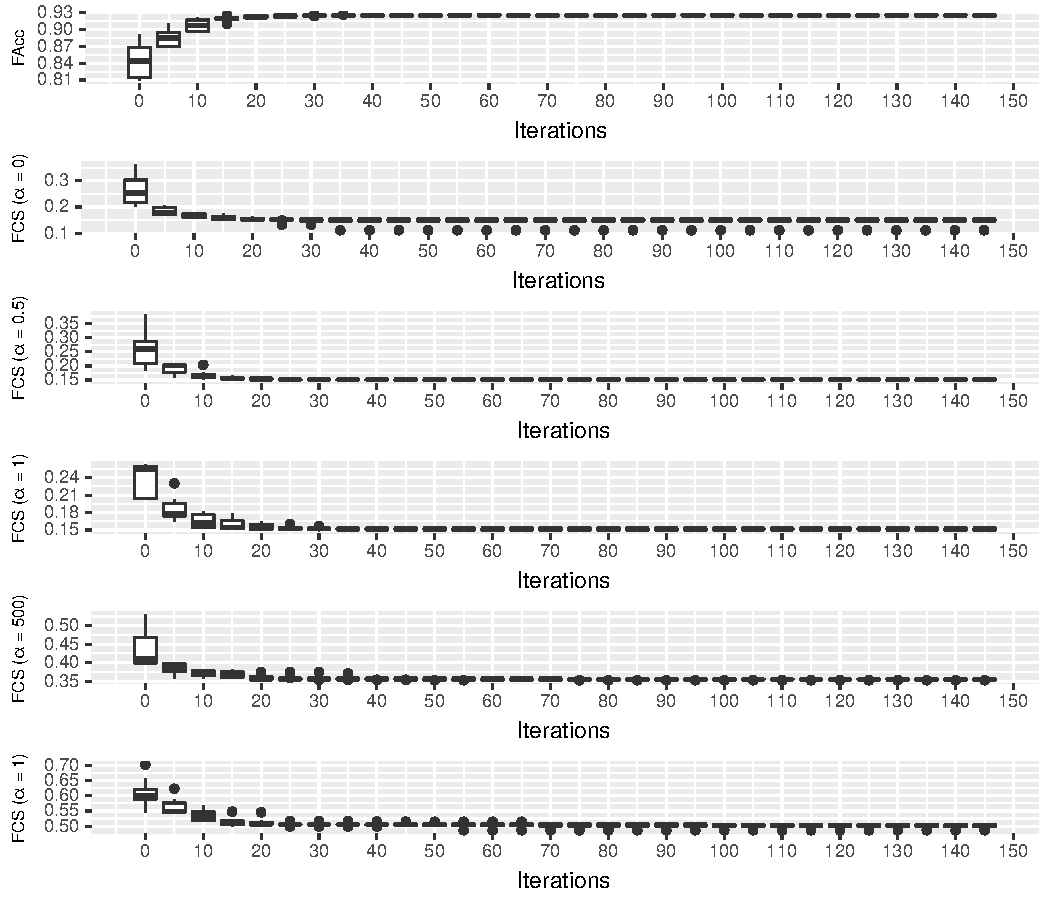
\includegraphics[width=0.8\textwidth]{img/pittsburghItvsF.pdf}
\caption{Convergence of fitness for each one of the tested fitness
  functions, and for Pittsburgh approach. Note that $f_{Acc}$ has to
  be maximised, whereas $f_{CS}$ has to be minimised.}
\label{fig:pittsburghItvsF}
\end{figure*}

For the sake of clarity, $f_{CS}$ has been divided by the maximum
value -- the number of instances for training -- it might take. By
looking at the Pittsburgh approach values in Figure
\ref{fig:pittsburghItvsF}, we show that mostly all configurations tend to converge around iteration 40, but it seems that $f_{CS}$ with
$\alpha = 0.5$ is the configuration that reaches the best solution
faster, around the 30th iteration.  

\begin{figure*}[h!tb]
	\centering
	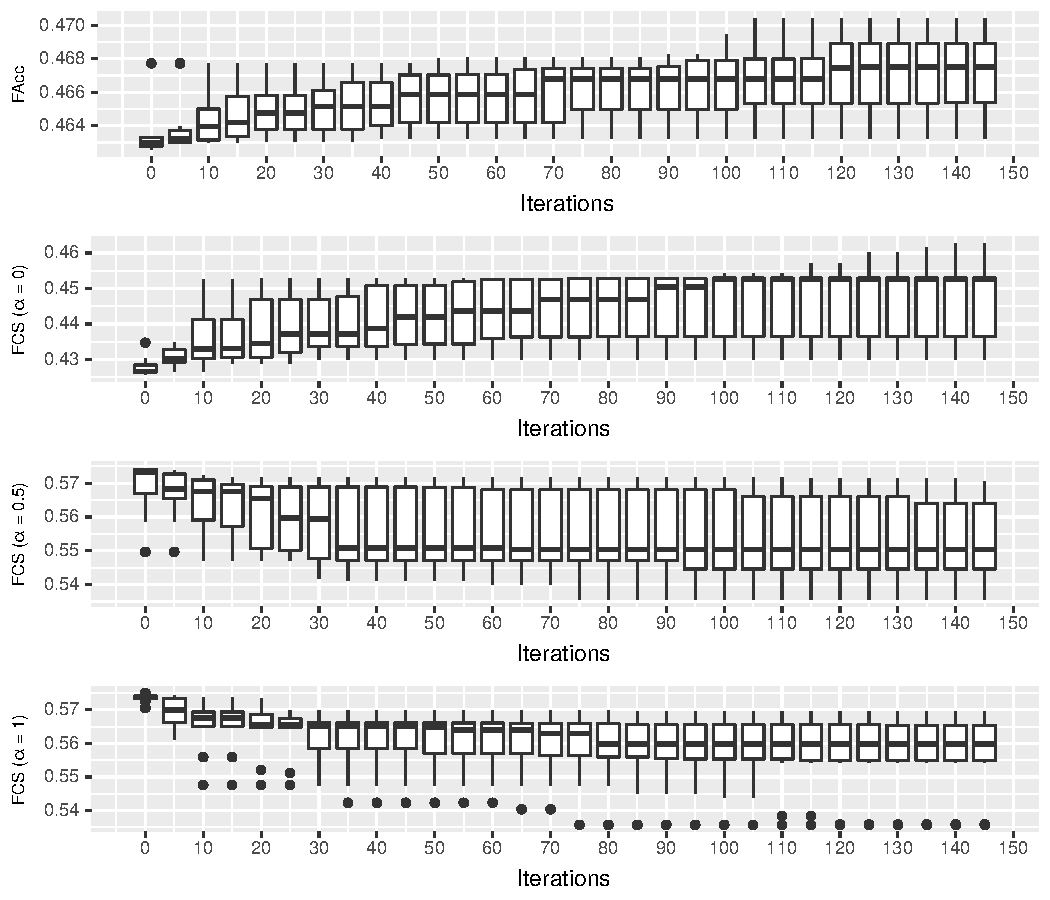
\includegraphics[width=0.8\textwidth]{img/michiganItvsF_allow.pdf}
	\caption{Convergence of fitness for each one of the tested fitness functions, and for Michigan approach being executed for the GRANTED class. Note that $f_{Acc}$ has to be maximised, whereas $f_{CS}$ has to be minimised.}
	\label{fig:michiganItvsF_allow}
\end{figure*}

With respect to the Michigan approach, a higher variability is noticeable in Figures \ref{fig:michiganItvsF_allow} and \ref{fig:michiganItvsF_deny}, but in average we see that for $f_{CS}$ with $\alpha = 0$ or 1, the fitness do not converge until generation 120. The best ones are for $f_{Acc}$ and $f_{CS}$ with $\alpha = 0.5$, being the latter the one that converges faster, around the 50th iteration.

\begin{figure*}[h!tb]
	\centering
	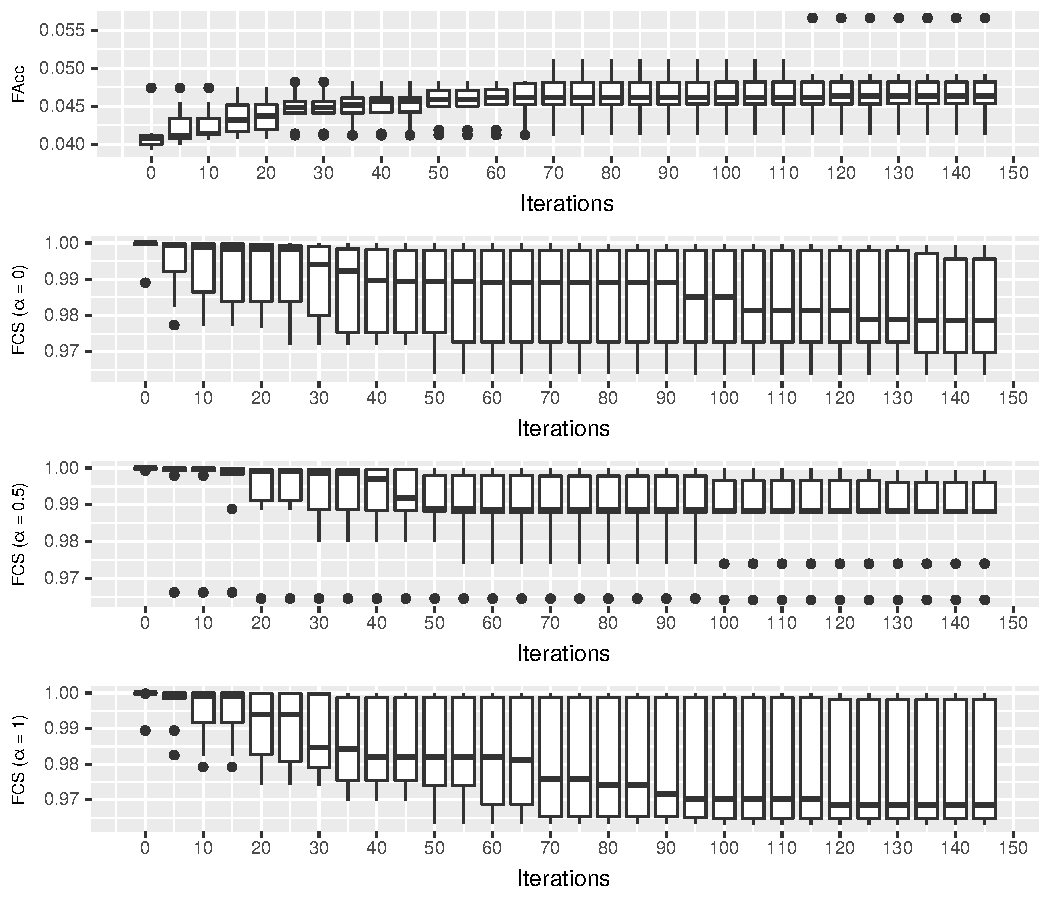
\includegraphics[width=0.8\textwidth]{img/michiganItvsF_deny.pdf}
	\caption{Convergence of fitness for each one of the tested fitness functions, and for Michigan approach being executed for the STRONGDENY class. Note that $f_{Acc}$ has to be maximised, whereas $f_{CS}$ has to be minimised.}
	\label{fig:michiganItvsF_deny}
\end{figure*}

We can advance that the best results might be obtained for $f_{CS}$
with $\alpha = 0.5$. However, there is a considerable difference between the performance, in terms of best
obtained fitness, of the two used approaches. In this way, we have to thoroughly compare them. In the next section we do so by chosing the validation coverage and the ratio of false positives and negatives as independent measurements. 

%\subsection{The Pittsburgh vs. Michigan approach} 
\label{subsec:approachcomparison}

Once the variability of the obtained fitness has been studied, and
always taking into account that those values come from their
evaluation in a training subset of the data, now we \textit{validate}
the proposed approaches with a validation set, similar to the validation set used in classification problems \cite{witten2005data}. 
 The way to evaluate this is similar to Equation \ref{eq:accuracy}, but using the validation subset of the data:

\begin{equation}
\label{eq:VALaccuracy}
v_{Acc} = (TP + TN) / T_{val}
\end{equation}

This measure will be the same independently of the approach or fitness
function has used to evaluate the individuals. Table
\ref{tab:PvsMvalidation} shows the average, best, median, and worst
results from the evaluations with $f_{Acc}$ and also $f_{CS}$. 

\begin{table}[h!]
	\centering
	\caption{Validation (accuracy in classification of a new
          dataset) scores for the Pittsburgh and Michigan approaches. \textbf{$*$} marks
          statistically significant best values.}
	\resizebox{13cm}{!}{
		\begin{tabular}{llll|l|l|l|l|l|l|}
			\cline{5-10}
			&  &  &  & \multicolumn{6}{l|}{Validation measurement} \\ 
			\cline{3-10} 
			& \multicolumn{1}{l|}{}  & \multicolumn{2}{l|}{Fitness function}  & Average & Best & Median & Worst & FP & FN \\
			\hline
			\multicolumn{2}{|l|}{\multirow{6}{*}{\begin{tabular}[c]{@{}l@{}}Pittsburgh:\\ Individual eq. set of rules\end{tabular}}}  & \multicolumn{2}{l|}{$f_{Acc}$}                                  & 0.925 $\pm$ 0.379e-2 & 0.929 & 0.926  & 0.917 & 0.075 $\pm$ 0.045e-1 & 0                    \\ \cline{3-10} 
			\multicolumn{2}{|l|}{}                                                                                                                                                                                                 & \multicolumn{1}{l|}{\multirow{3}{*}{$f_{CS}$}} & $\alpha$ = 0   & 0.926 $\pm$ 0.744e-2 & 0.945 & 0.926  & 0.917 & 0.072 $\pm$ 1.272e-2 & 0.002 $\pm$ 0.564e-2 \\ \cline{4-10} 
			\multicolumn{2}{|l|}{}                                                                                                                                                                                                 & \multicolumn{1}{l|}{}                          & $\alpha$ = 0.5 & 0.924 $\pm$ 0.371e-2 & 0.929 & 0.924  & 0.917 & 0.074 $\pm$ 0.451e-2 & 0 \\ \cline{4-10} 
			\multicolumn{2}{|l|}{}                                                                                                                                                                                                 & \multicolumn{1}{l|}{}                          & $\alpha$ = 1   & 0.925 $\pm$ 0.384e-2  & 0.929 & 0.926  & 0.917 & 0.075 $\pm$ 0.378e-2 & 0                    \\ \hline
			\multicolumn{1}{|l|}{\multirow{8}{*}{\begin{tabular}[c]{@{}l@{}}Michigan:\\ Individual eq. one rule\end{tabular}}} & \multicolumn{1}{l|}{\multirow{4}{*}{\begin{tabular}[c]{@{}l@{}}Class:\\ GRANTED\end{tabular}}}    & \multicolumn{2}{l|}{$f_{Acc}$}                                  & 0.467 $\pm$ 0.143e-2 & 0.472 & 0.468  & 0.459 & 0.023 $\pm$ 0.095e-1 & 0                    \\ \cline{3-10} 
			\multicolumn{1}{|l|}{}                                                                                             & \multicolumn{1}{l|}{}                                                                             & \multicolumn{1}{l|}{\multirow{3}{*}{$f_{CS}$}} & $\alpha$ = 0   & 0.466 $\pm$ 0.441e-2 & 0.472 & 0.467  & 0.459 & 0.021 $\pm$ 0.094e-1 & 0                    \\ \cline{4-10} 
			\multicolumn{1}{|l|}{}                                                                                             & \multicolumn{1}{l|}{}                                                                             & \multicolumn{1}{l|}{}                          & $\alpha$ = 0.5 & 0.467 $\pm$ 0.305e-2 & 0.472 & 0.467  & 0.462 & 0.019 $\pm$ 0.088e-1 & 0                    \\ \cline{4-10} 
			\multicolumn{1}{|l|}{}                                                                                             & \multicolumn{1}{l|}{}                                                                             & \multicolumn{1}{l|}{}                          & $\alpha$ = 1   & 0.465 $\pm$ 0.43e-2  & 0.472 & 0.467  & 0.458 & 0.023 $\pm$ 0.099e-1 & 0                    \\ \cline{2-10} 
			\multicolumn{1}{|l|}{}                                                                                             & \multicolumn{1}{l|}{\multirow{4}{*}{\begin{tabular}[c]{@{}l@{}}Class:\\ STRONGDENY\end{tabular}}} & \multicolumn{2}{l|}{$f_{Acc}$}                                  & 0.046\textbf{$*$} $\pm$ 0.74e-2  & 0.065 & 0.045  & 0.037 & 0 & 0.307 $\pm$ 0.745e-1 \\ \cline{3-10} 
			\multicolumn{1}{|l|}{}                                                                                             & \multicolumn{1}{l|}{}                                                                             & \multicolumn{1}{l|}{\multirow{3}{*}{$f_{CS}$}} & $\alpha$ = 0   & 0.025 $\pm$ 1.527e-2 & 0.045 & 0.023  & 0.003 & 0 & 0.004 $\pm$ 0.039e-1 \\ \cline{4-10} 
			\multicolumn{1}{|l|}{}                                                                                             & \multicolumn{1}{l|}{}                                                                             & \multicolumn{1}{l|}{}                          & $\alpha$ = 0.5 & 0.02 $\pm$ 1.603e-2  & 0.061 & 0.015  & 0.002 & 0 & 0.007 $\pm$ 0.063e-1 \\ \cline{4-10} 
			\multicolumn{1}{|l|}{}                                                                                             & \multicolumn{1}{l|}{}                                                                             & \multicolumn{1}{l|}{}                          & $\alpha$ = 1   & 0.025 $\pm$ 1.948e-2 & 0.047 & 0.036  & 0     & 0 & 0.004 $\pm$ 0.049e-1 \\ \hline
		\end{tabular}
	}
	\label{tab:PvsMvalidation}
\end{table}

In Section \ref{subsec:fitnesscomparison} we have shown that the performance in the
fitness of the Michigan approach was worse than that of Pittsburgh,
and now it is more clear, given that the accuracy over the validation set is
not even 50\%. In fact, the dataset we are using is highly imbalanced; there are 1 instance
in the training set of data labelled as STRONGDENY for every 13
labelled as GRANTED. Thus, the results we have obtained are biased towards the majority
class \cite{japkowicz2002class}. 

At the same time, and because the distributions for the Michigan approach follow the normal, an ANOVA test has been performed in every class \cite{DerracTests11}, obtaining a p-value of 0.5538 for the GRANTED class, meaning that there are not statistically significant differences in the results. However, in the case of the STRONGDENY class, using $f_{CS}$ significantly (p-value of 0.001736) decreases the accuracy over the validation set. With regard to how many FP and FN are obtained in every approach, we see in Table \ref{tab:PvsMvalidation} that for the Pittsburgh approach we generally obtain low rates or 0 -- ideal -- false negatives, and around 7\% rate of false positives -- almost 400 in average for our validation set --. On the other hand, best rates are found for the Michigan approach, where the rate of FP is, at most, 2.8\% -- around 113 instances in average --. And even if there were FN found, the average for the used validation set is 29 instances out of 5330, which is a very low number and as we explained before, in this BYOD scenario it is less worse to have FN than FP. Also, this imbalance in the FP and FN values is also caused by the imbalance in the dataset.

% Esta se deja comentada por si piden más resultados

%\begin{table*}
%\centering
%\resizebox{16.5cm}{!}{
%\begin{tabular}{llll|l|l|l|l|l|l|}
%\cline{5-10}
%  &  &  &  & \multicolumn{6}{l|}{Validation measurement} \\ 
%  \cline{3-10} 
%  & \multicolumn{1}{l|}{}  & \multicolumn{2}{l|}{Fitness function}  & Average & Best & Median & Worst & FP & FN \\
%  \hline
%\multicolumn{2}{|l|}{\multirow{6}{*}{\begin{tabular}[c]{@{}l@{}}Pittsburgh:\\ Individual eq. set of rules\end{tabular}}}  & \multicolumn{2}{l|}{$f_{Acc}$}                                  & 0.925 $\pm$ 0.379e-2 & 0.929 & 0.926  & 0.917 & 0.075 $\pm$ 0.045e-1 & 0                    \\ \cline{3-10} 
%\multicolumn{2}{|l|}{}                                                                                                                                                                                                 & \multicolumn{1}{l|}{\multirow{3}{*}{$f_{CS}$}} & $\alpha$ = 0   & 0.926 $\pm$ 0.744e-2 & 0.945 & 0.926  & 0.917 & 0.072 $\pm$ 1.272e-2 & 0.002 $\pm$ 0.564e-2 \\ \cline{4-10} 
%\multicolumn{2}{|l|}{}                                                                                                                                                                                                 & \multicolumn{1}{l|}{}                          & $\alpha$ = 0.5 & 0.924 $\pm$ 0.371e-2 & 0.929 & 0.924  & 0.917 & 0.074 $\pm$ 0.451e-2 & 0 \\ \cline{4-10} 
%\multicolumn{2}{|l|}{}                                                                                                                                                                                                 & \multicolumn{1}{l|}{}                          & $\alpha$ = 1   & 0.925 $\pm$ 0.384e-2  & 0.929 & 0.926  & 0.917 & 0.075 $\pm$ 0.378e-2 & 0                    \\ \cline{4-10}
%\multicolumn{2}{|l|}{}                                                                                                                                                                                                 & \multicolumn{1}{l|}{}                          & $\alpha$ = 500   & 0.867 $\pm$ 0.337e-2  & 0.871 & 0.867  & 0.86 & 0.07 $\pm$ 0.382e-2 & 0                    \\ \cline{4-10}
%\multicolumn{2}{|l|}{}                                                                                                                                                                                                 & \multicolumn{1}{l|}{}                          & $\alpha$ = 1000   & 0.867 $\pm$ 0.438e-2  & 0.871 & 0.868  & 0.859 & 0.066 $\pm$ 0.772e-2 & 0                    \\ \hline
%\multicolumn{1}{|l|}{\multirow{8}{*}{\begin{tabular}[c]{@{}l@{}}Michigan:\\ Individual eq. one rule\end{tabular}}} & \multicolumn{1}{l|}{\multirow{4}{*}{\begin{tabular}[c]{@{}l@{}}Class:\\ GRANTED\end{tabular}}}    & \multicolumn{2}{l|}{$f_{Acc}$}                                  & 0.467 $\pm$ 0.143e-2 & 0.472 & 0.468  & 0.459 & 0.023 $\pm$ 0.095e-1 & 0                    \\ \cline{3-10} 
%\multicolumn{1}{|l|}{}                                                                                             & \multicolumn{1}{l|}{}                                                                             & \multicolumn{1}{l|}{\multirow{3}{*}{$f_{CS}$}} & $\alpha$ = 0   & 0.466 $\pm$ 0.441e-2 & 0.472 & 0.467  & 0.459 & 0.021 $\pm$ 0.094e-1 & 0                    \\ \cline{4-10} 
%\multicolumn{1}{|l|}{}                                                                                             & \multicolumn{1}{l|}{}                                                                             & \multicolumn{1}{l|}{}                          & $\alpha$ = 0.5 & 0.467 $\pm$ 0.305e-2 & 0.472 & 0.467  & 0.462 & 0.019 $\pm$ 0.088e-1 & 0                    \\ \cline{4-10} 
%\multicolumn{1}{|l|}{}                                                                                             & \multicolumn{1}{l|}{}                                                                             & \multicolumn{1}{l|}{}                          & $\alpha$ = 1   & 0.465 $\pm$ 0.43e-2  & 0.472 & 0.467  & 0.458 & 0.023 $\pm$ 0.099e-1 & 0                    \\ \cline{2-10} 
%\multicolumn{1}{|l|}{}                                                                                             & \multicolumn{1}{l|}{\multirow{4}{*}{\begin{tabular}[c]{@{}l@{}}Class:\\ STRONGDENY\end{tabular}}} & \multicolumn{2}{l|}{$f_{Acc}$}                                  & 0.046 $\pm$ 0.74e-2  & 0.065 & 0.045  & 0.037 & 0 & 0.307 $\pm$ 0.745e-1 \\ \cline{3-10} 
%\multicolumn{1}{|l|}{}                                                                                             & \multicolumn{1}{l|}{}                                                                             & \multicolumn{1}{l|}{\multirow{3}{*}{$f_{CS}$}} & $\alpha$ = 0   & 0.025 $\pm$ 1.527e-2 & 0.045 & 0.023  & 0.003 & 0 & 0.004 $\pm$ 0.039e-1 \\ \cline{4-10} 
%\multicolumn{1}{|l|}{}                                                                                             & \multicolumn{1}{l|}{}                                                                             & \multicolumn{1}{l|}{}                          & $\alpha$ = 0.5 & 0.02 $\pm$ 1.603e-2  & 0.061 & 0.015  & 0.002 & 0 & 0.007 $\pm$ 0.063e-1 \\ \cline{4-10} 
%\multicolumn{1}{|l|}{}                                                                                             & \multicolumn{1}{l|}{}                                                                             & \multicolumn{1}{l|}{}                          & $\alpha$ = 1   & 0.025 $\pm$ 1.948e-2 & 0.047 & 0.036  & 0     & 0 & 0.004 $\pm$ 0.049e-1 \\ \hline
%\end{tabular}
%}
%\caption{Comparison between Pittsburgh and Michigan
%  approaches, in terms of their validation scores. Validation has been calculated as the accuracy in classifying a test dataset. An $*$ indicates
%  the  statistically significant best value for $\alpha$.}
%\label{tab:PvsMvalidation}
%\end{table*}

To evaluate computation costs of the two approaches, and taking into consideration the infrastructure available for the experiments (see Section\ref{sec:experiments}), we present the execution times in Table \ref{tab:PvsMtime}, detailed by their average value and standard deviation, along weith the best, worst, and median values. Time is expressed in hours, for the sake of clarification. In addition, the values for the Michigan approach are not separated by class this time, because in order to have the two rules - one for each class -- the CSO would have to wait for both executions.
%
\begin{table*}[h!tbp]
	\centering
	\caption{Execution time, Pittsburgh and Michigan approaches;
          this one adds times for GRANTED and STRONGDENY. \textbf{$*$} marks  statistically significant best values.}
	\resizebox{10.5cm}{!}{
	\begin{tabular}{lll|l|l|l|l|}
		\cline{4-7}
		&                                                &                & \multicolumn{4}{l|}{Time measurement (h)}     \\ \cline{2-7} 
		\multicolumn{1}{l|}{}                                                                                                    & \multicolumn{2}{l|}{Fitness function}                           & Average            & Best   & Median & Worst  \\ \hline
		\multicolumn{1}{|l|}{\multirow{4}{*}{\begin{tabular}[c]{@{}l@{}}Pittsburgh:\\ Individual eq. set of rules\end{tabular}}} & \multicolumn{2}{l|}{$f_{Acc}$}                                  & 18.371 $\pm$ 7.178 & 8.545  & 17.366 & 31.366 \\ \cline{2-7} 
		\multicolumn{1}{|l|}{}                                                                                                   & \multicolumn{1}{l|}{\multirow{3}{*}{$f_{CS}$}} & $\alpha$ = 0   & 14.424 $\pm$ 2.938 & 7.016 & 14.352  & 17.43 \\ \cline{3-7} 
		\multicolumn{1}{|l|}{}                                                                                                   & \multicolumn{1}{l|}{}                          & $\alpha$ = 0.5\textbf{$*$} & 11.934 $\pm$ 2.22 & 8.267  & 11.609  & 16.166 \\ \cline{3-7} 
		\multicolumn{1}{|l|}{}                                                                                                   & \multicolumn{1}{l|}{}                          & $\alpha$ = 1   & 13.176 $\pm$ 1.923 & 9.283 & 13.424 & 16.517 \\ \hline
		\multicolumn{1}{|l|}{\multirow{4}{*}{\begin{tabular}[c]{@{}l@{}}Michigan:\\ Individual eq. one rule\end{tabular}}}       & \multicolumn{2}{l|}{$f_{Acc}$}                                  & 10.627 $\pm$ 0.187 & 10.307 & 10.64  & 10.956 \\ \cline{2-7} 
		\multicolumn{1}{|l|}{}                                                                                                   & \multicolumn{1}{l|}{\multirow{3}{*}{$f_{CS}$}} & $\alpha$ = 0\textbf{$*$}   & 9.342 $\pm$ 0.3    & 8.993  & 9.261  & 9.854  \\ \cline{3-7} 
		\multicolumn{1}{|l|}{}                                                                                                   & \multicolumn{1}{l|}{}                          & $\alpha$ = 0.5 & 9.435 $\pm$ 0.348  & 9.039  & 9.401  & 10.281 \\ \cline{3-7} 
		\multicolumn{1}{|l|}{}                                                                                                   & \multicolumn{1}{l|}{}                          & $\alpha$ = 1   & 9.612 $\pm$ 0.508  & 8.946  & 9.509  & 10.38  \\ \hline
	\end{tabular}
}
	\label{tab:PvsMtime}
\end{table*}

In this table we see that best times are obtained when $f_{CS}$ is used. More precisely, in the Pittsburgh approach, the distributions follow the normal and after performing the ANOVA test, we can say that the shorter execution time (the best) is found for $\alpha$ = 0.5 with statistical significance (p-value of 0.008623). In the case of the Michigan approach, we again find statistical differences (p-value of 5.537e-05) between the results, and thus we can say that the best execution time is obtained when we use $f_{CS}$ with an $\alpha$ value of 0. It seems that the time does decrease when $\alpha$ is different than 0, meaning that the depth of the tree is taken into account during the evaluation of the fitness. To study this effect, we have to look at the sizes of the best individuals obtained for each configuration, which are displayed in Table \ref{tab:PvsMsize}.

\begin{table*}[h!tb]
	\centering
	\caption{Tree size of the best individuals for the Pittsburgh approach. An \textbf{$*$} indicates the  statistically significant best value for $\alpha$.}
	\resizebox{10.5cm}{!}{
	\begin{tabular}{lll|l|l|l|l|}
		\cline{4-7}
		&                                                &                & \multicolumn{4}{l|}{Best individual size}     \\ \cline{2-7} 
		\multicolumn{1}{l|}{}                                                                                                    & \multicolumn{2}{l|}{Fitness function}                           & Average            & Best   & Median & Worst  \\ \hline
		\multicolumn{1}{|l|}{\multirow{4}{*}{\begin{tabular}[c]{@{}l@{}}Pittsburgh:\\ Individual eq. set of rules\end{tabular}}} & \multicolumn{2}{l|}{$f_{Acc}$}                                  & 60.2 $\pm$ 10.922 & 47 & 60 & 79 \\ \cline{2-7} 
		\multicolumn{1}{|l|}{}                                                                                                   & \multicolumn{1}{l|}{\multirow{3}{*}{$f_{CS}$}} & $\alpha$ = 0   & 60 $\pm$ 11.086 & 43 & 60 & 83 \\ \cline{3-7} 
		\multicolumn{1}{|l|}{}                                                                                                   & \multicolumn{1}{l|}{}                          & $\alpha$ = 0.5 & 40 $\pm$ 4.447 & 35 & 40  & 47 \\ \cline{3-7} 
		\multicolumn{1}{|l|}{}                                                                                                   & \multicolumn{1}{l|}{}                          & $\alpha$ = 1\textbf{$*$}   & 36.2 $\pm$ 3.011 & 31 & 37 & 39 \\ \hline
	\end{tabular}
	}
	\label{tab:PvsMsize}
\end{table*}

In this table we only show the results for the Pittsburgh approach, given that the sizes of the trees do change in GP, but the size of a list -- number of conditions in the rule -- does not, and in this case is always 10. Certainly, the size of the trees diminishes when the value of $\alpha$ grows. Since the distributions do not follow the normal, a non-parametric test (Kruskal-Wallis) has been used to asset the statistical significance \cite{DerracTests11}, obtaining a p-value of 1.679e-10. Then, the smaller individual is found for $f_{CS}$, and $\alpha$ = 1.

% Esta se deja comentada por si piden más resultados

%\begin{table*}
%\centering
%\begin{tabular}{lll|l|l|l|l|}
%\cline{4-7}
%                                                                                                                         &                                                &                & \multicolumn{4}{l|}{Time measurement (h)}     \\ \cline{2-7} 
%\multicolumn{1}{l|}{}                                                                                                    & \multicolumn{2}{l|}{Fitness function}                           & Average            & Best   & Median & Worst  \\ \hline
%\multicolumn{1}{|l|}{\multirow{4}{*}{\begin{tabular}[c]{@{}l@{}}Pittsburgh:\\ Individual eq. set of rules\end{tabular}}} & \multicolumn{2}{l|}{$f_{Acc}$}                                  & 18.371 $\pm$ 7.178 & 8.545  & 17.366 & 31.366 \\ \cline{2-7} 
%\multicolumn{1}{|l|}{}                                                                                                   & \multicolumn{1}{l|}{\multirow{3}{*}{$f_{CS}$}} & $\alpha$ = 0   & 14.424 $\pm$ 2.938 & 7.016 & 14.352  & 17.43 \\ \cline{3-7} 
%\multicolumn{1}{|l|}{}                                                                                                   & \multicolumn{1}{l|}{}                          & $\alpha$ = 0.5 & 11.934 $\pm$ 2.22 & 8.267  & 11.609  & 16.166 \\ \cline{3-7} 
%\multicolumn{1}{|l|}{}                                                                                                   & \multicolumn{1}{l|}{}                          & $\alpha$ = 1   & 13.176 $\pm$ 1.923 & 9.283 & 13.424 & 16.517 \\ \cline{3-7}
%\multicolumn{1}{|l|}{}                                                                                                   & \multicolumn{1}{l|}{} & $\alpha$ = 500   & 3.653 $\pm$ 0.36 & 3.239 & 3.576 & 4.436 \\ \cline{3-7}
%\multicolumn{1}{|l|}{}                                                                                                   & \multicolumn{1}{l|}{} & $\alpha$ = 1000   & 3.256 $\pm$ 0.229 & 2.922 & 3.284  & 3.624 \\ \hline
%\multicolumn{1}{|l|}{\multirow{4}{*}{\begin{tabular}[c]{@{}l@{}}Michigan:\\ Individual eq. one rule\end{tabular}}}       & \multicolumn{2}{l|}{$f_{Acc}$}                                  & 10.627 $\pm$ 0.187 & 10.307 & 10.64  & 10.956 \\ \cline{2-7} 
%\multicolumn{1}{|l|}{}                                                                                                   & \multicolumn{1}{l|}{\multirow{3}{*}{$f_{CS}$}} & $\alpha$ = 0   & 9.342 $\pm$ 0.3    & 8.993  & 9.261  & 9.854  \\ \cline{3-7} 
%\multicolumn{1}{|l|}{}                                                                                                   & \multicolumn{1}{l|}{}                          & $\alpha$ = 0.5 & 9.435 $\pm$ 0.348  & 9.039  & 9.401  & 10.281 \\ \cline{3-7} 
%\multicolumn{1}{|l|}{}                                                                                                   & \multicolumn{1}{l|}{}                          & $\alpha$ = 1   & 9.612 $\pm$ 0.508  & 8.946  & 9.509  & 10.38  \\ \hline
%\end{tabular}
%\caption{Comparison between Pittsburgh and Michigan
%  approaches, in terms of their execution time. For the Michigan approach, times for executing the algorithm once for the GRANTED class and another for the STRONGDENY are presented together. An $*$ indicates the  statistically significant best value for $\alpha$.}
%\label{tab:PvsMtime}
%\end{table*}


% \subsection{Examples of the best obtained individuals}
% \label{subsec:examples}

What we also have to determine is which kind of presented solution is
better: showing the CSO a set of rules or a single rule for each
class.
%
% As already discussed in Section \ref{sec:methodology}, each one has their advantages and disadvantages, but now we directly compare some of the best individuals obtained for both implementations, proving their readability and usefulness for the CSOs. In addition, we present the relation between the obtained solutions and the original rules that allowed to classify the dataset we have been working with.
%
% As we have executed the experiments performing a 10-fold
% cross-validation, in order to study the best individuals for each
% configuration we need to consider the values of the validation
% accuracies per fold, and then choose the best one.
Figure \ref{fig:bestInd_fCS_a0} shows an example of best individual
obtained using $f_{CS}$ and $\alpha = 0 $. The tree in this figure represents a set of 16 rules, two of them classifying to the STRONGDENY class, whilst the rest classify towards the GRANTED class. The ones that classify to STRONGDENY have been highlighted and presented in string form in the figure.

\begin{figure*}[h!tb]
	\centering
	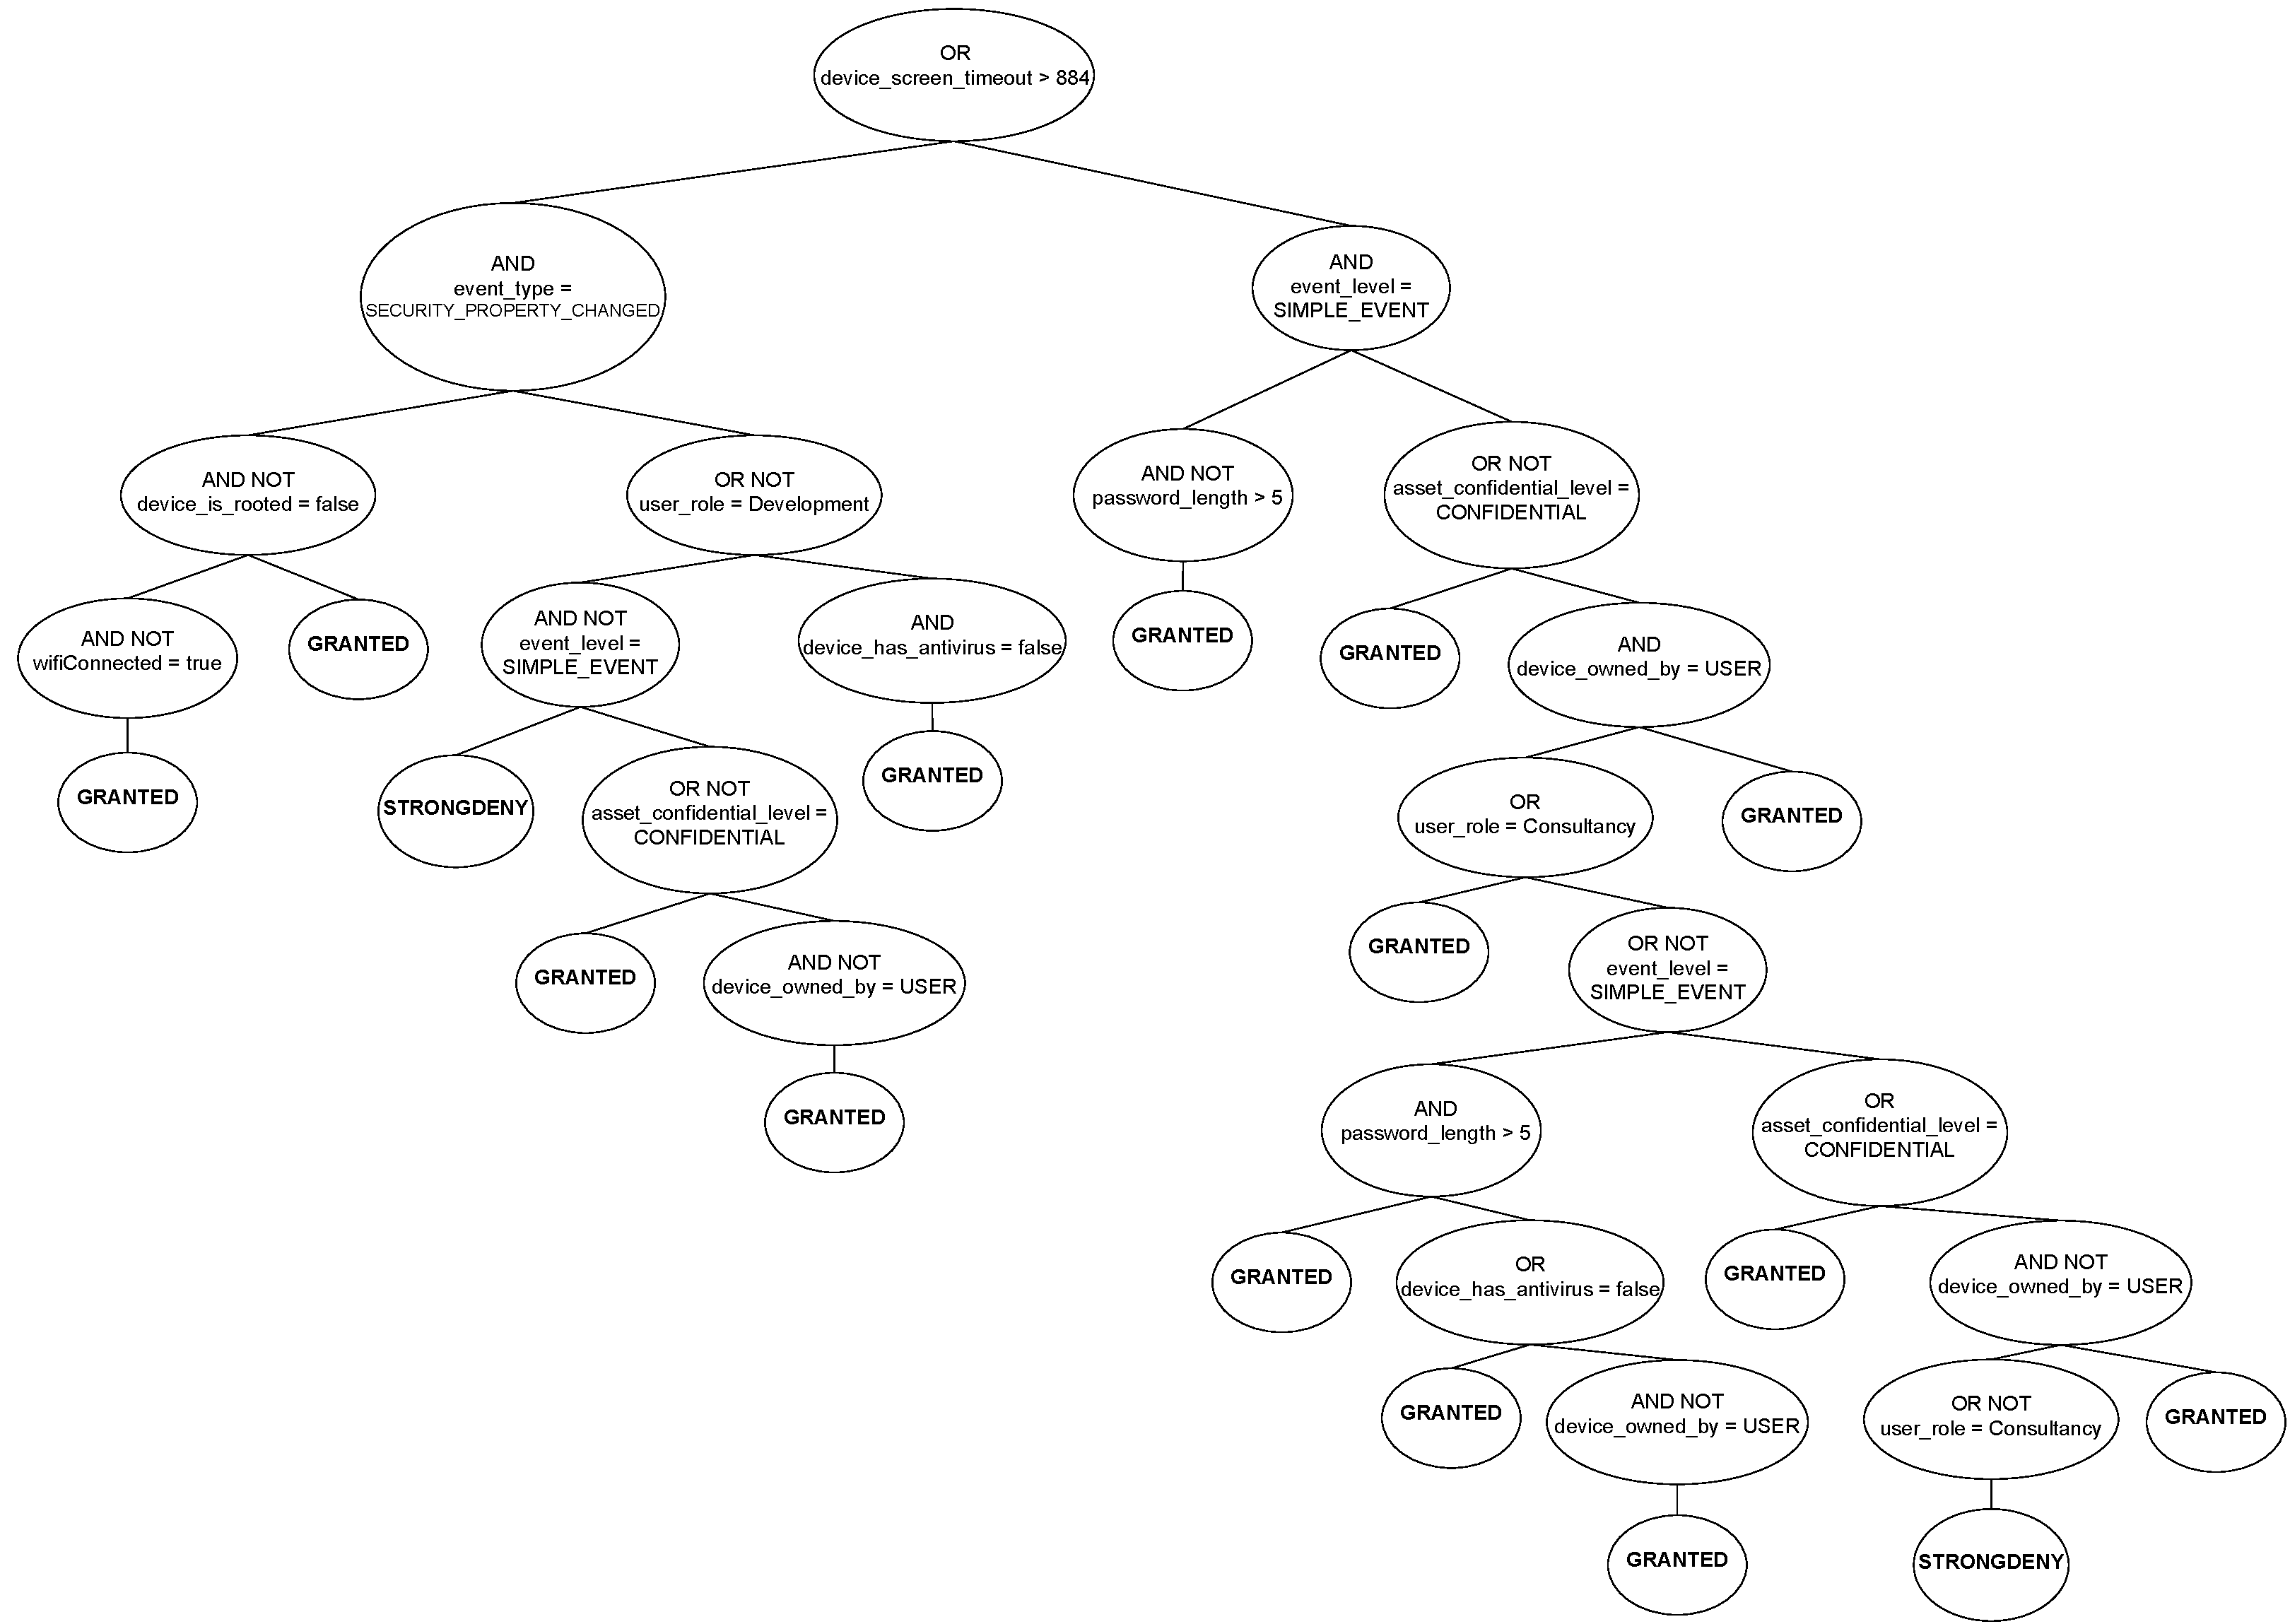
\includegraphics[width=\textwidth]{img/bestInd_fCS_a0.pdf}
	\caption{Example with $f_{CS}$ and $\alpha=0$.} 
	\label{fig:bestInd_fCS_a0}
\end{figure*}

The STRONGDENY rules in Figure \ref{fig:bestInd_fCS_a0} imply that
the developers are more probably to get a GRANTED in their actions,
and this conclusion makes sense because because they are supposed to
be more familiar with system security. Also, from the second rule we
can infer that the complex events -- not simple -- and the BYOD
devices imply a certain degree of unsafety. The root, and thus most important, condition, is related to the time that the the device takes to enter into sleep mode (screen turns off). 

% In general, what we have seen in the individuals obtained by the
% Pittsburgh approach is that most of the rules in the set classify for
% the GRANTED class, and less than 13\% are classifying for the
% STRONGDENY class. Again, the effect of the imbalance in the dataset is
% present. Actually, in some cases the set of rules only classify to
% GRANTED, and this can be seen as a ``whitelist'', meaning that
% everything that is not specify by these rules will be automatically
% denied.

% %Maybe some comment on the root rule, which is the most discriminating
% %one. Or some insight from the rules you could give the CSO - JJ

\section{Conclusions and Future Work}
\label{sec:future}

% General layout of conclusions
% We wanted to do this with this motivation.
% We have done this and that in this paper and met objective 1 and 2 or answered research question 1 and 2; however, we think that question 3 has not been answered properly
% We think we could answer question 3 properly if we did this and that. Which is left as future work.

In this work, we wanted to help companies adopting the BYOD philosophy
by developing a tool that is able to discover rules using a GP
approach, from the users behaviour when interacting with their
devices, at the time it minimises the false positives, so that a
dangerous action is never taken as permitted. To this end, in Section \ref{sec:methodology} we have
presented different ways to implement a methodology based on GP, by two
approaches: Pittsburgh, in which the individuals are coded as set or
rules; and Michigan, where the individuals are a single rule, and thus
a rule for every class has to be generated. In addition, two different
fitness functions have been used to study their effect over the
validation accuracy rate and the number of false positives and
negatives.

The results in Section \ref{sec:gp} make a fine proof of concept of a tool that helps the CSO of a company discovering dangerous situations through the presentation of GP generated rules. We obtained promising rates for the number of false positives (around
7\%), and good coverage over the validation data set is shown in
Section \ref{subsec:approachcomparison}. However, since the ideal
value for both false positives and negatives is 0, there is room for
improvement. In addition, Figure \ref{fig:bestInd_fCS_a0} shows
that the individuals are presented in a readable form, but the ratio
between rules classifying to one or another class is too much biased
towards the GRANTED class. %We need to get this back, now there's
                           %space for it.

With regard to the execution time, the solution we propose takes between 16 and 17 hours, in the worst case and taking into account the used infrastructure, to obtain the best individual. Although these times could be acceptable, in the sense that the CSO would have new rules everyday, they can still be reduced.  
                                % Was it a challenge for GP? In which
                                % way?
                                % (Paloma) Yes? Maybe? Hope so? I don't know :( Pablo what do you think? 
% What follows is future work %Pablo: yes, I would move this paragraph at the end, and maybe add again the references you mentioned earlier in section 4.2
A possible way to
achieve better values for FP and FN is to set up the problem as a
multiobjective one, so that we try to minimise $f_{CS}$, but also FP
and FN. Additionally we will try to reduce the execution time by adapting the algorithm parameters, for instance, the number of generations, as has been shown in Section \ref{subsec:fitnesscomparison} that in some cases 50 generations is enough. Other enhancements could be to study every tree individual and to directly not evaluate the fitness for the contradictory rules of each one. 

On the other hand, the imbalance of the dataset should be taken into
account, given that it affects to the results in terms of obtained
accuracy in the validation process and the ratio among classes in the
obtained individuals. Solutions can be found in literature in order to reduce the bias while performing classification
tasks, such as in \cite{chawla2005data} and \cite{sun2009classification}. Another typical way of approaching this problem is to
use balancing techniques over the data, such as ``oversampling'' \cite{smote_02}, in
which sintetic instances of the minority class -- STRONGDENY -- are
created and introduced in the dataset, until there are approximately
the same number of instances than in the majority class -- GRANTED
--. Also, in \cite{bhowan2012developing}, the authors present a comparison between many different types of
fitness functions, testing on various unbalanced datasets, with
different minority-class/majority-class ratios.

For our future work we will implement these solutions to continue
improving our system. Furthermore, we will extend the approach to other problems where data is available. For example, particularisations of the BYOD problem as it could be Internet navigation during work hours. We will explore network traffic from public data repositories, such as \url{http://www.secrepo.com/#3p\_network}, and try to apply our approach. 

\section{Acknowledgements}

Acks taking\\
this much space.

\bibliographystyle{splncs04}      
\bibliography{GPrules,geneura}   

\end{document}


